%%
%% This is file `sample-authordraft.tex',
%% generated with the docstrip utility.
%%
%% The original source files were:
%%
%% samples.dtx  (with options: `authordraft')
%% 
%% IMPORTANT NOTICE:
%% 
%% For the copyright see the source file.
%% 
%% Any modified versions of this file must be renamed
%% with new filenames distinct from sample-authordraft.tex.

%% 
%% For distribution of the original source see the terms
%% for copying and modification in the file samples.dtx.
%% 
%% This generated file may be distributed as long as the
%% original source files, as listed above, are part of the
%% same distribution. (The sources need not necessarily be
%% in the same archive or directory.)
%%
%% The first command in your LaTeX source must be the \documentclass command.
\documentclass[sigconf]{acmart}
\usepackage{mathtools, xcolor, colortbl, booktabs, dcolumn, caption, siunitx, tabularx}
\usepackage{multirow}
\usepackage{acronym, amsmath}

%%
%% \BibTeX command to typeset BibTeX logo in the docs
\AtBeginDocument{%
  \providecommand\BibTeX{{%
    \normalfont B\kern-0.5em{\scshape i\kern-0.25em b}\kern-0.8em\TeX}}}

%% Rights management information.  This information is sent to you
%% when you complete the rights form.  These commands have SAMPLE
%% values in them; it is your responsibility as an author to replace
%% the commands and values with those provided to you when you
%% complete the rights form.
\setcopyright{rightsretained}
\copyrightyear{2020}
\usepackage[utf8]{inputenc}

%% These commands are for a PROCEEDINGS abstract or paper.
\acmConference[Forschungsseminar 19/20]{Forschungsseminar}{March 9, 2020}{Regensburg, DE}
\acmBooktitle{Regensburg 20: Forschungsseminar,
  March, 2020, Regensburg, DE}

%%
%% Submission ID.
%% Use this when submitting an article to a sponsored event. You'll
%% receive a uniuue submission ID from the organizers
%% of the event, and this ID should be used as the parameter to this command.
%%\acmSubmissionID{123-A56-BU3}

%%
%% The majority of ACM publications use numbered citations and
%% references.  The command \citestyle{authoryear} switches to the
%% "author year" style.
%%
%% If you are preparing content for an event
%% sponsored by ACM SIGGRAPH, you must use the "author year" style of
%% citations and references.
%% Uncommenting
%% the next command will enable that style.
%%\citestyle{acmauthoryear}

%%
%% end of the preamble, start of the body of the document source.
\begin{document}

%%
%% The "title" command has an optional parameter,
%% allowing the author to define a "short title" to be used in page headers.
\title{Faster than in Real ime \\
- \\
Prediction of Human Motions in Virtual Reality }

%%
%% The "author" command and its associated commands are used to define
%% the authors and their affiliations.
%% Of note is the shared affiliation of the first two authors, and the
%% "authornote" and "authornotemark" commands
%% used to denote shared contribution to the research.
\author{Andreas Pfaffelhuber}
\email{andreas.pfaffelhuber@stud.uni-regensburg.de }
\affiliation{%
  \institution{Universität Regensburg}
  \city{Regensburg}
  \state{Deutschland}
}

\author{Christoph Tögel}
\email{christoph.toegel@stud.uni-regensburg.de}
\affiliation{%
  \institution{Universität Regensburg}
  \city{Regensburg}
  \state{Deutschland}
}

\author{Julian Dietz}
\email{julian.dietz@stud.uni-regensburg.de}
\affiliation{%
  \institution{Universität Regensburg}
  \city{Regensburg}
  \state{Deutschland}
}

%%
%% By default, the full list of authors will be used in the page
%% headers. Often, this list is too long, and will overlap
%% other information printed in the page headers. This command allows
%% the author to define a more concise list
%% of authors' names for this purpose.
\renewcommand{\shortauthors}{Pfaffelhuber, Tögel \& Dietz}

\begin{abstract}
Experiences in Virtual Reality (VR) strongly depend on the immersion of the user in the computer generated world.
Hardware delays and a resulting asynchrony from real world motions to the virtual motions can induce motion sickness and overall a worse experience.
Using machine learning on motion capture data, a user's motions can be predicted and shown in advance.
In this study an apparatus to improve VR experiences by reducing delays or even present user's their future motions is proposed.
Therefore experience in VR is evaluated using subjective and objective measures on a two-dimensional, multidirectional Fitts' law task.
In the study 24 participants wearing full body motion capture suits were presented different motion alterations with past, present and multiple future versions of their motions.
Performance was evaluated using a standardized Fitts' law task under six conditions as well as using three questionnaires for subjective measures. 
Initially expected improvements of performance as well as experience could not be found, but a worsening of both measures was observed.
\end{abstract}

%%
%% The abstract is a short summary of the work to be presented in the
%% article.

%%
%% The code below is generated by the tool at http://dl.acm.org/ccs.cfm.
%% Please copy and paste the code instead of the example below.
%%

%%\begin{teaserfigure}
%%  \includegraphics[width=\textwidth]{sampleteaser.pdf}
%%  \caption{Motive and Unity showing 3D skeletons}
%%  \Description{Screenshots of both Motive and Unity showing the 3D skeleton of a %%detected participant}
%%  \label{fig:teaser}
%%\end{teaserfigure}

%%
%% Keywords. The author(s) should pick words that accurately describe
%% the work being presented. Separate the keywords with commas.
\keywords{virtual reality, neural networks, motion prediction, embodiment, presence, Fitts law}

%%
%% This command processes the author and affiliation and title
%% information and builds the first part of the formatted document.
\maketitle

\section{Introduction}\label{tit:Introduction}
When users move their limbs in Virtual Reality (VR) through active and voluntary motoric motions and the brains expected outcome positions match the received sensory afferent modalities like gaze and proprioception, a strong VR-Illusion is perceived~\cite{Gonzalez-Franco2017}.
Contrary, if the difference between the afferent sensory inputs and the expected outcome position is too big, the virtual limb-ownership illusion is often rejected by users~\cite{Gonzalez-Franco2017}.
Several studies in the field of VR experiences have demonstrated that body ownership illusion is induced with visuo-motor triggers when both real and fake bodies move their homologous body parts at the same time~\cite{Banakou2013, Kilteni2013}.
Similarly, it has been observed that the body ownership illusion fails to be established when either temporal synchronicity~\cite{Shimada2010} or spatial congruence~\cite{Dummer2009} between the seen and the felt motions are not met. 
As shown above, the perceived plausibility of ones body perception and its congruency with motions in the virtual reality environment is of great importance for immersive experiences.
To prevent a delay of one’s virtual body motion through hardware-based factors, the current body motion can be used to predict the future position of limbs. 
Systems capable of predicting a user's motions are able to remove the hardware delay of the displayed virtual body, or even take the prediction one step further and present the user with a position that is still located in the future. 
This modified version of the motion allows for a faster task completion as it may better represent a users intention when interacting in the virtual space.\\

In an attempt to solve this problem, motion data has been recorded from 20 participants in a previous study performing prescribed and free form tasks .
This motion data describes a skeleton consisting of 51 bones and positional data. 
Neural networks can be trained on this data to compute a different version of the skeleton, which is evaluated in this study.
Depending on the input data this can be done for multiple time offsets in the past or future.
The effect of the time offsets on user experience and motions can be measured objectively and subjectively.
The final user performance will be measured as the throughput on a standardized Fitts' law tapping task~\cite{A2004} presented in VR, as already established in other related work~\cite{Schwind2019a}. 
This study aims to compare the user's performance, presence, avatar embodiment and acceptance of the proposed system at different \textsc{prediction time offsets} in virtual reality.
This approach expects to find a certain \textsc{prediction time offset} which produces an observable maximum in user performance, presence as well as avatar embodiment and thus provides a better VR experience.\\ 

The following paper presents related work for virtual body alteration and limb ownership, motion prediction and Fitts' law performance evaluations. Building on previous works we use an objective, quantitative method to evaluate body alterations as well as the user's subjective feedback. The proposed Fitts' law task allows to compute throughput as a performance measure. Our findings show a worsening of performance depending on the strength of alteration of a user's motions contrary to initial expectations. While the results do not support the hypothesis, this study indicates a correlation between alteration and performance. The performance never plateaus which might be caused by the apparatus and not by the motion prediction. As noted in later sections the used apparatus was limited by available hardware and constrained to a certain approach when defining the neural network architecture. Therefore the observed effect might be inverted to a performance increase when lifting these.

\section{Related Work}\label{tit:RelatedWork}
The related work covers findings on avatar embodiment and limb ownership as well as previous body alteration studies and their effect on the presence felt within a virtual environment. 
Since it is a main theme of this study, related work on the effects of differences between displayed and real limb positions is presented. 
Additionally, a quick overview on Fitts' law and its meaning for human computer interaction is given as it is later used to quantitively measure performance of conditions.

\subsection{Virtual Limb Ownership}
The concept of body ownership refers to the sense that one's own body is the source of sensations. It involves a strong afferent component that indicates the state of the body through various peripheral signals and is not only present while performing voluntary actions, but also during inactive experiences~\cite{Tsakiris2006}.
Similarly, the sense of embodiment refers to the ensemble of sensations that arise in conjunction with being inside, having, and controlling a body~\cite{Kilteni2012}.
The concept of presence describes the sense of being in the virtual world rather than still consciously being in the real physical world~\cite{Sanchez-vives2005}.
Since body ownership refers to the form of identification with the body as a whole, limb-ownership refers to only certain parts of the body~\cite{Braun2018}.

The "rubber-hand illusion"~\cite{Botvinick2006} shows that alien limbs can be perceived as being a part of the own body through perception and simultaneous tactile stimulation of a fake and real hand.
Similar findings have been made concerning the adaptation of virtual limbs or bodies.
Perez-Marcos et al. induced a virtual hand ownership illusion and showed that some aspects of the illusion occur through motor imagery used to control movements of the virtual hand.
When the movements of the virtual hand followed motor imagery, the illusion of ownership of the virtual hand was evoked and measured muscle activity correlated with movements of the virtual arm~\cite{Perez-Marcos2009}.

Considering the topic of perceived limb ownership in a virtual environment, Rietzler et al. conducted a study that works with direct manipulation of limb positions~\cite{Rietzler2018a}.
Their goal was to simulate weight in the virtual reality by slightly displacing the subjects virtual arm position and thus for example forcing them to lift their arm higher than usual if an object should be heavier. 
Pure visual displacement is used instead of a physical actuator allowing for modification based on software only. 
While weights could only be simulated in a relative manner, the approach showed to have positive effects on the user experience, leading to much higher presence and immersion during the use of the apparatus~\cite{Rietzler2018a}.
Adjusting the virtually displayed limb positions generally suggests to be a viable approach since in VR, visual cues can overshadow haptic impressions under certain conditions. 
For example, Kohli~\cite{Kohli2010} built an apparatus which mapped real world touches to visual feedback by snapping virtual limbs onto virtual object representations in order to align the haptic sensation.
This improved the experience only up to a certain threshold as the visual cues did overshadow haptic impressions.
Visual displacement of the virtual body position can also be used to simulate slow-motion in a VR environment, and has also shown to be accepted by the participants under this condition.
Proving this, another one of Rietzler's works~\cite{Rietzler2018} explored virtual limb-transformation in the past time direction, slowing down motions and using previously captured data instead of predicted future data like this current study aims to. 
Using multiple Microsoft Kinect V2 cameras and a virtual environment, multiple filters were deployed to compute the slowed motion, allowing for a dynamic slow-motion experience.  
The strength of this effect is linked to the velocity of motions by the participant~\cite{Rietzler2018}. 
In a game of hitting bubbles no decrease in presence could be found.
This may be caused by the user-controlled nature of the slow-motion effect, but also indicates once again that users accept adjustments of their virtual body position.

\subsection{Motion prediction}
Another study using limb-manipulation was conducted by Kasahara et al.~\cite{Kasahara2017}, who developed a system that captures full-body motions and generates estimated past and future body positions using a time-based alteration model where the amount of temporal shift could be adjusted as a continuous value.
 They investigated how human movement and the user's observable behavior change according to the virtual body alterations.
Results showed that spatial-temporal alteration of a virtual body results in perceivable changes of the physical feeling as well as physical movement. For example a virtual human body generated at approximately 25-100 milliseconds in the future induced a "lighter weight" sensation~\cite{Kasahara2017}.

Other works in the context of predicting motions in virtual reality have already been conducted, many of them centering around predicting the user's head movement. 
While some approaches include creating and examining algorithmic methods towards this goal~\cite{Aladagli2018}, others follow a similar approach as this study and use neural networks. In one case, both recurrent and time delayed neural networks have been used to predict the future head position, and both prediction systems have shown to be usable and provide adequate results ~\cite{Saad} in the virtual reality context.

The state-of-the-art approach of using machine learning to predict movement has already shown to be able to enhance the user's performance in multiple scenarios, for example when using a touchscreen in a non-virtual, two-dimensional paradigm \cite{Le2017}.

Considering the successful application in such a scenario as well as the shown applicability of the same method within virtual reality environments~\cite{Saad}, we decided to also use machine learning to predict the user's motions and alter their virtual body position accordingly.
The presented related work already tried similar fashioned approaches and managed to enable the user to have a better virtual immersion or to create new experiences in the virtual world.
The now conducted study and its used apparatus try to enable the motion prediction approach for the entire virtual body in a three-dimensional, virtual environment and aim to improve performance in selection tasks as well as the immersive experience. 

\subsection{Fitts' Law}
To objectively compare the overall performance of selection tasks during the study, a standardized Fitts' law task is used.
Fitts' law ~\cite{Information1954} itself is an information-theoretic view of human motor behavior which expresses the time to complete a movement task (\textit{MT}) in terms of distance or amplitude of the move (\textit{A}) and the width of the region within which the move must terminate (\textit{W}).
With the intercept (\textit{a}) and the slope (\textit{b}), the performance of a pointing device can be evaluated ~\cite{Mackenzie1989}.
Fitts' law over the years has been verified over a wide range of conditions and has been applied by HCI researchers in primarily two ways. 
Firstly, it can be used as a predictive model to e.g. calculate the estimated time for the user of a graphical interface to move the mouse tracker to a button and click on it. 
Secondly, it is used for the comparison and evaluation of novel pointing devices or conditions ~\cite{A2004}. 
Instead of predicting movement times, researchers measure several of them and then determine how the different conditions and devices affect the coefficients within the Fitts' law relation. 
Fitts' law offers the utility to compress several movement time measurements into a single statistic, the throughput.
Throughput combines both speed and accuracy, and its value in describing input devices and conditions has been both academically and industrially recognized~\cite{A2004}.

\subsection{Summary}
The presented work shows an overall interest in modifying human motions in virtual environments in order to significantly alter or improve the user experience. 
The related work on virtual limb ownership demonstrates that displacements influence the user experience and might be used to enhance the virtual experience due to often being accepted by the user, as long as the displacements are not making too drastic changes to the body position. 
This study now focuses on evaluating the use of deep learning to create prediction models for future motions. It also focuses on quantifying the results and experience of the displacements with standardized measures. 
As mentioned above, neural networks have already shown that they are capable of improving user performance in a two dimensional scenario, so applying them in a virtual, three-dimensional environment might yield similar results.
To test this the conducted study evaluates how participants perform a standardized Fitts' law task, which is widely recognized and used by the scientific community.

\section{General Method}\label{section:General_Method}
In this paper an evaluation study of different \textsc{prediction time offsets} for predicting human motions using a horizontal, two-dimensional, multidirectional Fitts' law task in a virtual environment is conducted.
In order to record user motion data we use a full-body motion capture system (OptiTrack) with its proprietary "Motive" recording software at version 2.1.1.
During the study participants wear a full-body motion capture suit with 49 passive markers.
As even small motions can be dependent on bigger bone and muscle structures it is necessary to capture the whole body.
Due to imprecision of a finer marker setup, only an abstract marker configuration for hands is used. With this only the thumb, index finger and pinkie are captured with the remainders interpolated.

\begin{figure}[H]
  \centering
  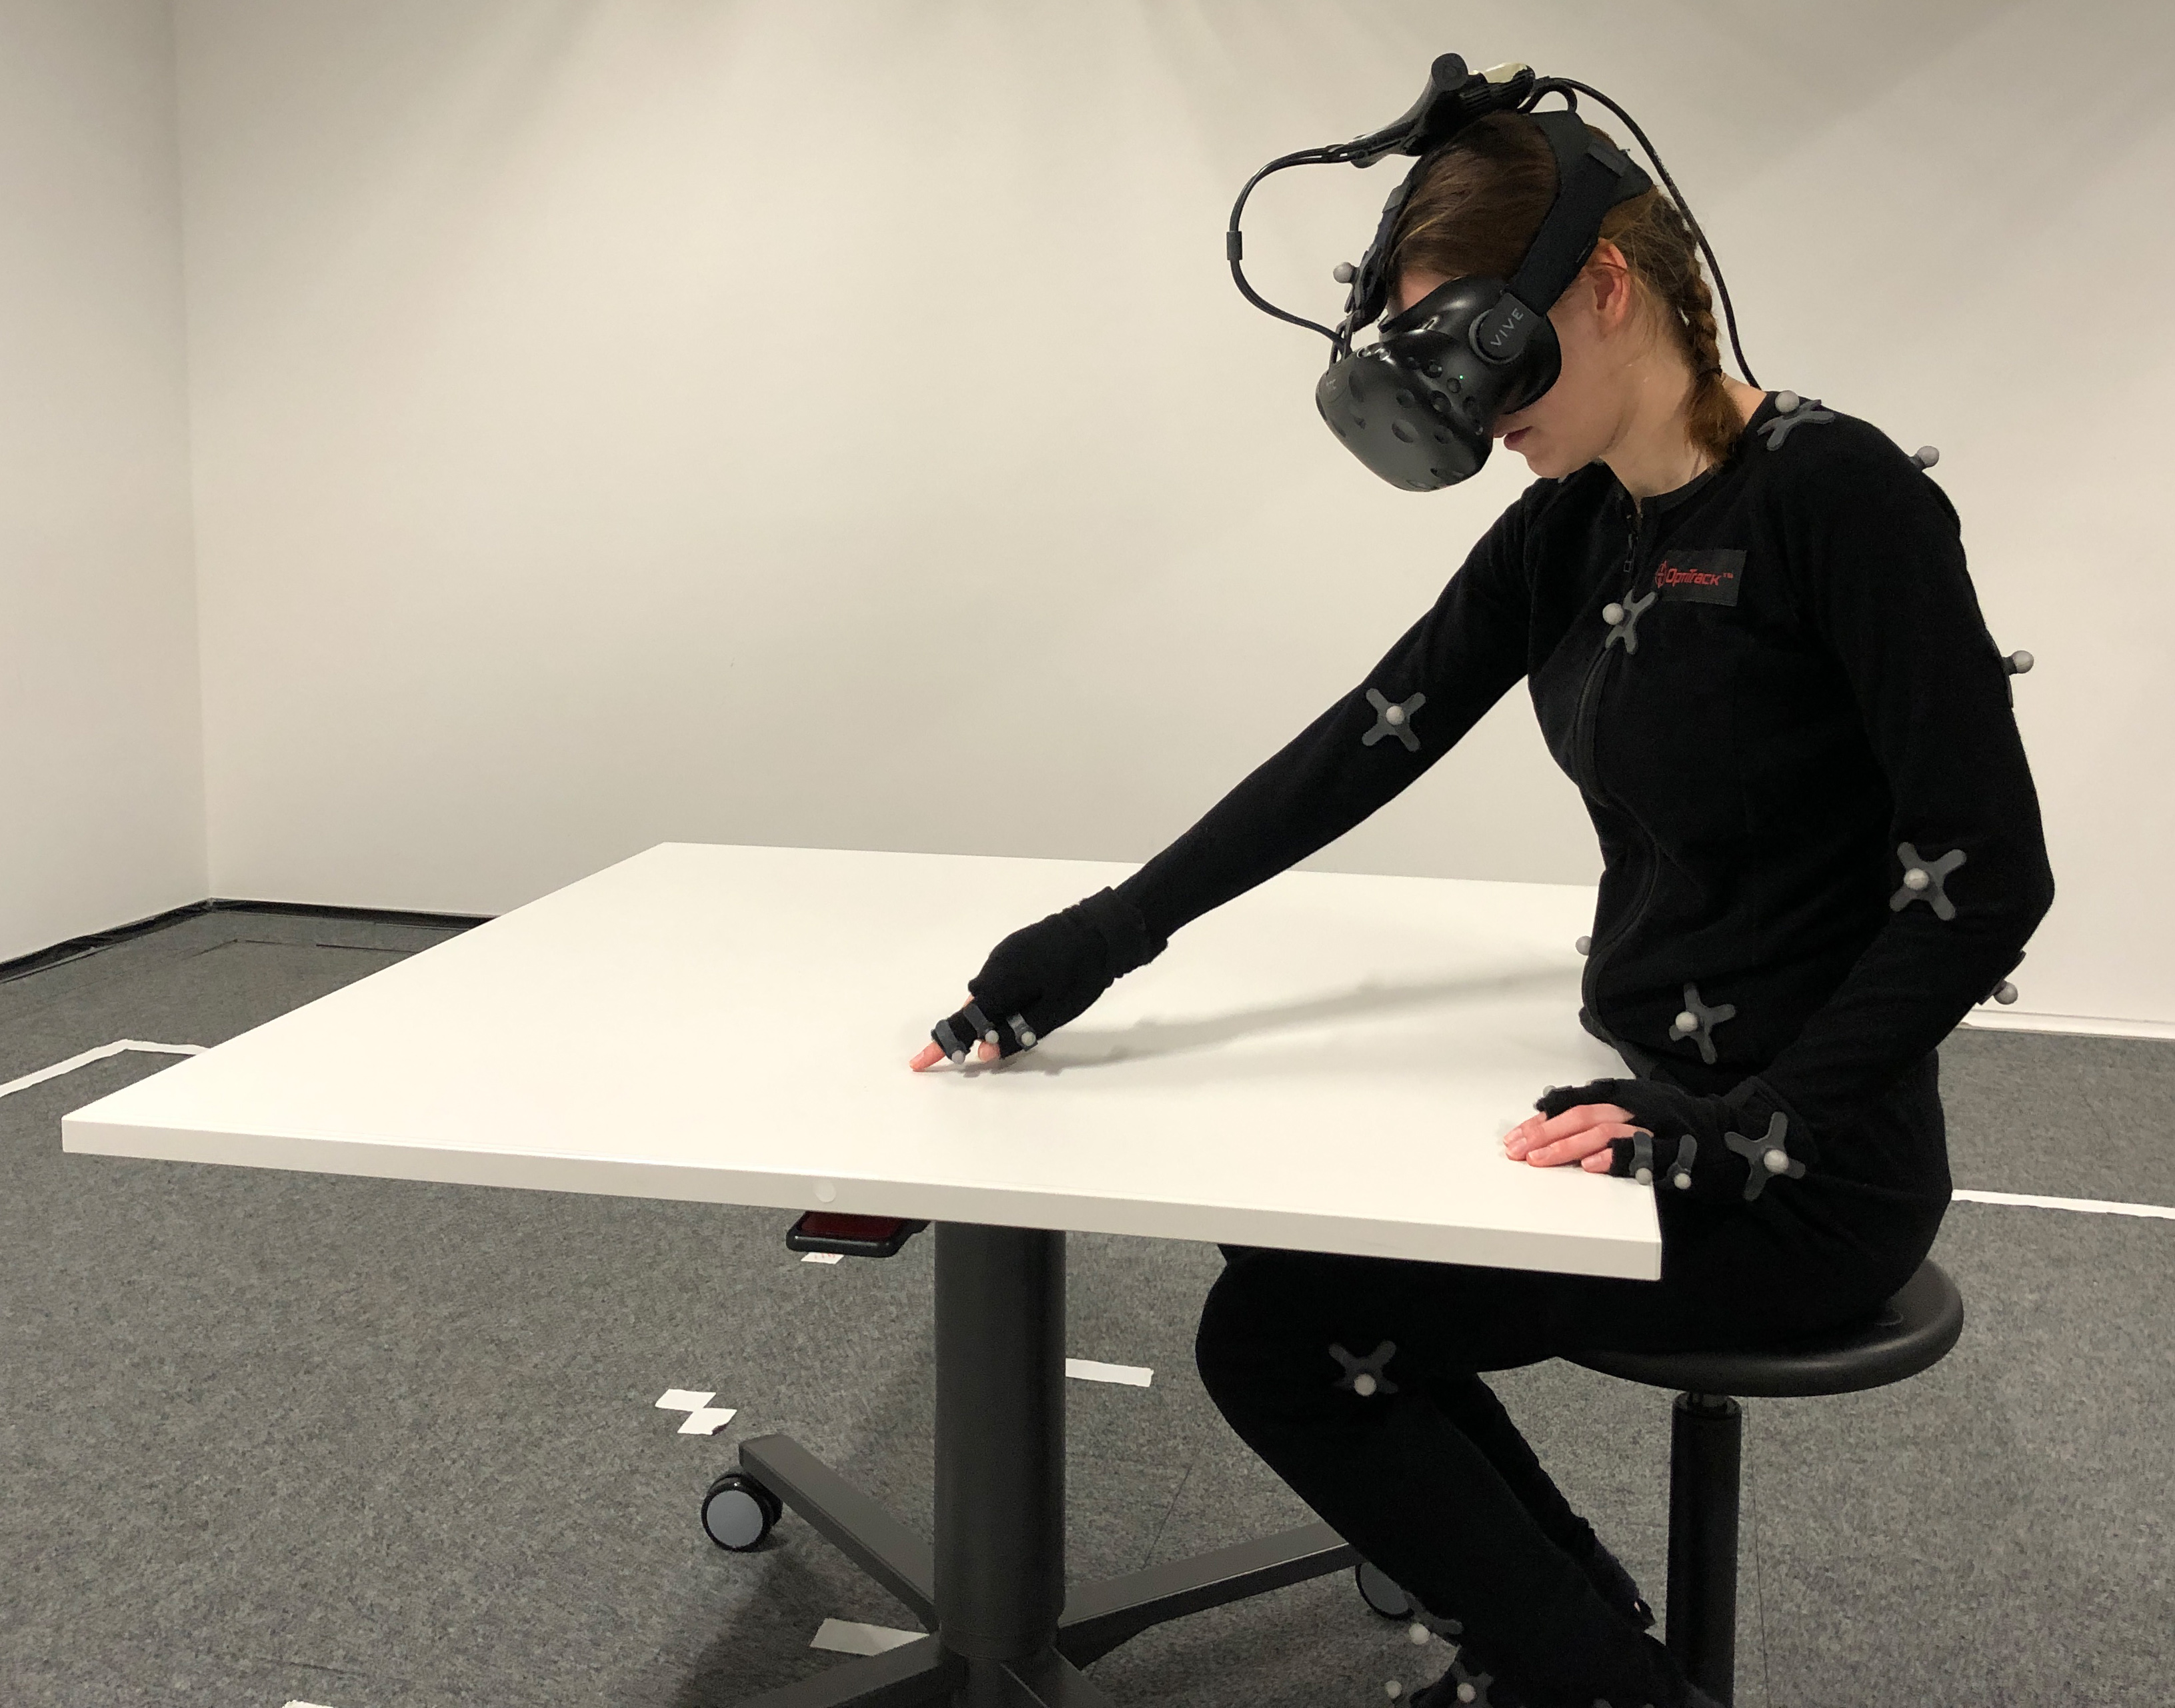
\includegraphics[width=0.5\linewidth]{PT_}
  \caption{Participant performing the Fitts' law task wearing a full-body motion capturing suit.}
  \Description{Participant performing the Fitts' law task wearing a full-body motion capturing suit.}
  \label{fig:PT_}
\end{figure}

\subsection{Prediction Times Determination}
The tested \textsc{prediction time offsets} in this experiment have been determined from pervious experiences with the apparatus. The latency of the base system caused by hardware was determined, which is used as the first offset towards predicting a future version. Apart from this condition that eliminates the hardware delay through the used \textsc{prediction time offset}, three additional ones are located in the future. All \textsc{prediction time offsets} then use the same time interval between them, so that the resulting models can be linearly compared. Additionally the \textit{base system} without any prediction is evaluated as a condition. As the sixth condition a \textit{past time model} is used. This condition differs from the future ones, as it does not use an algorithm to determine motions but rather presents buffered data from the user. It has the same offset as the \textit{zero latency model} but in the other time direction. This way it can be evaluated how performance changes according to the different \textsc{prediction time offsets} compared to the \textit{base system}.
The \textit{past time model} allows to calculate a regression model along the different evaluations and serves as a plausibility check.
The different conditions can be seen in table~\ref{table:tableTimePredictionOffsets}.

\begin{table}
\caption{Time prediction offsets used in the study.}
\begin{tabular}{ccc} 
\hline
	Name & Frames & Prediction Time [ms] \\
\hline
Past model &  -12 & -48 \\ 
Base system & 0 & 0 \\
Zero Latency model & +12 & +48 \\
Future model 2 & +24 & +96 \\
Future model 3 & +36 & +144 \\
Future model 4 & +48 & +192 \\
\hline
\end{tabular}
\label{table:tableTimePredictionOffsets}
\end{table}

Four future prediction models have been chosen so that some of the models should over-predict the user's motions up to a point where performance starts to decline again. This leads to the expectation to model a user's performance more detailed.

\subsection{Evaluation Study}
The hypothesis of the evaluation study is that different \textsc{prediction time offsets} will have an effect on user performance, presence and avatar embodiment. These are expected to increase from the past model until a slightly-in-the-future model and then decrease again. 
To test this hypothesis, the evaluation study will be conducted using a within-subjects design that consists of six different \textsc{prediction time offsets}. For each condition participants first perform the Fitts' law task and then answer three questionnaires, as well as some qualitative questions orally. The six \textsc{prediction time offsets} are evaluated using a 6 $\times$ 6 counterbalanced latin square design. The system is tested on 24 participants, which is similar to other studies in the same context~\cite{Kasahara2017, Rietzler2018}.

Using G*Power the size of the sample was evaluated. This study conducted a within-factors repeated measures design. Therefore, assuming a significance level of 5 percent ($\alpha$ = .05) and a power of 95 percent , even a small effect size of Cohen's \textit{d} (.3) could be observed. This results in a minimum of 20 required participants~\cite{Faul2007, Erdfelder2009}. In order to align with the latin squared design the sample was extended to 24 participants. 

\subsection{Fitts' Law Design}\label{sec:FittsLaw}
The user performance will be measured quantitatively using the throughput of a standardized, two-dimensional multidirectional Fitts' law tapping task for each condition. 
The entire task is laid out according to the established recommendations by Soukoreff and Mackenzie ~\cite{A2004}, which go in accordance with and supplement the ISO 9241-9:2000.
This norm has been revised by ISO 9241-400:2007 and ISO 9241-411:2012.
The task consists of a circular arrangement of multiple round targets, which then have to be tapped by the participant (See figure~\ref{fig:FittsLawUnity_}). These are displayed on a horizontal virtual desk.  The procedure always starts with the upper middle target, then the target at the opposite side of the circle is chosen next. This way the participant taps clockwise through the circle.

\begin{figure}[H]
  \centering
  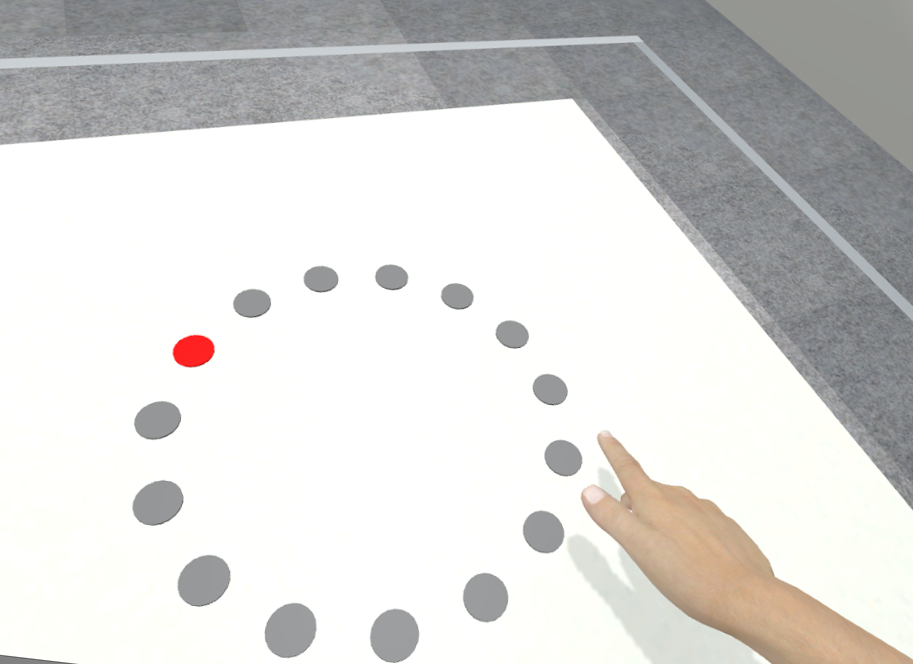
\includegraphics[width=0.5\linewidth]{FittsLawUnity_}
  \caption{Participant performing the Fitts' law task in the virtual environment.}
  \Description{Participant performing the Fitts' law task in the virtual environment.}
  \label{fig:FittsLawUnity_}
\end{figure}

In our study two repetitions of nine different Fitts' law circle configurations (3 target sizes(\textit{W}) $\times$ 3 target distances(\textit{D})) are performed.
 Every circle consists of 15 clickable targets, and participants thus perform 288 taps per \textsc{prediction time offset} condition.
 According to acknowledged recommendations~\cite{A2004} and a similar setup by Schwind et al.~\cite{Schwind2019}, this setup captures sufficient data to compare the different conditions. 
The different configurations appear randomly ordered for each condition. 
The targets are big enough to be precisely activated using the virtual index finger (\textit{W}), the distances cover the whole table (\textit{D}). 
To compute the initial index of difficulty (\textit{ID}) for the different circle configurations the Shannon formulation is used, which offers an improved link with information theory as well as better correlations compared to other models proposed by Welford or Fitts~\cite{Mackenzie1989, 10.5555/143848}.

The employed setup covers indexes of difficulty for the different configurations that range from 2.26 to 4.83 bits, which roughly compares to general recommendations~\cite{A2004} as well as previous related work~\cite{Schwind2019}. 
While participants perform the Fitts' law task, multiple quantitative measures are captured to evaluate their performance during the different movement conditions. Movement times as well as a measure of the scatter of the participants' movement is gathered. For this, we log the physical end-points of each movement task.\\

\subsection{Questionnaires}\label{sec:Questionnaires}

Presence as well as embodiment are evaluated using both the igroup presence questionnaire (iPQ)~\cite{Schubert1999} and an avatar embodiment questionnaire~\cite{Gonzalez-Franco2018}. The iPQ is a widely used tool in the field of VR evaluation and was developed and refined over a multitude of studies~\cite{Regenbrecht2002, Schubert2001, Schubert2002}.

The avatar embodiment questionnaire was created by Gonzalez-Franco and Peck~\cite{Gonzalez-Franco2018} in an attempt to provide a standardized questionnaire to measure embodiment.
Since it has multiple sub-scales the questionnaire was shortened down to three, namely "body ownership", "agency and motor control" and "location of the body". 
These scales are also weighted highest by the original authors~\cite{Gonzalez-Franco2018} and are the only applicable ones for this setup. 
For a shallow investigation of motion sickness another questionnaire is presented, though only the four most significant questions named by the authors~\cite{Gianaros2001} are used.
For the study all questionnaires are shown after each \textsc{prediction time offset} in randomized ordering of their respective questions using an online survey tool. The participants leave the virtual environment in order to fill them out on a laptop.
Furthermore six question which can be answered in a free-from manner are asked after the questionnaires: 

 \begin{itemize}
 \item Wie hat sich dein Körper während dieses Durchlaufs angefühlt?
 (How did your body feel during this iteration?)
 \item Was ist dir allgemein hierbei aufgefallen?
 (What did you notice during this iteration?)
 \item War diese Erfahrung positiv oder negativ?
 (Was this experience positive or negative for you?)
 \item Hast du einen Unterschied zu den bisherigen Läufen bemerkt?
 (Did you notice a difference in regards to the other iterations?)
 \item Konntest du deine Auswahl präzise treffen?
 (Were you able to chose your targets precisely )
 \item Wie hat sich der digitale Avatar angefühlt~?
 (How did the digital avatar feel to you?)
 \end{itemize}
 
 These questions are presented verbally in German as all participants were native speakers.

\subsection{Procedure}
Participants are first welcomed and asked to fill out an informed consent form as well as a demographics survey.
They are told that they will be testing different motion tracking configurations while performing the Fitts' law task described in section~\ref{sec:FittsLaw} followed by multiple questionnaires and free-form questions. They are instructed to use their right hand index finger for this. 
Participants don't know about the motion prediction and are thus expected to not be biased in their impressions. Participants are additionally informed that their participation is on a purely free basis and that they can abort the experiment at any given time if they wish to. The volunteer then take on their motion suit and head-mounted display (HMD) to enter an VR replica of the laboratory. They then are presented the first of the \textsc{prediction time offsets} and perform the Fitts' law task followed by the used questionnaires and the free-from questions. They are allowed to take a short break after each condition, repeating the process until all six conditions are completed. At the end the participant is thanked for taking part in the study and is compensated.

\subsection{Sample}
The study consisted of 24 participants (13 Males, 11 Females). All participants were right-handed with the exception of one. The mean age was 23.21 years-old (\textit{SD} = 3.24 years).
Participants were either wearing contact lenses, took their glasses off or were comfortable with wearing them underneath the HMD. Students were compensated with credit points, which resembled most of the test subjects. Remaining participants got sweets. Additionally the height of the students was recorded with the average being 1.77 meters tall (\textit{SD} = .08 m). Neither of the participants reported to have much previous experience using virtual reality devices. 

\section{Apparatus}\label{tit:Apparatus}
\subsection{Motion capturing system}
In order to record user motion data we use the motion capture system (OptiTrack\footnote{https://optitrack.com}) with the proprietary "Motive" application (version 2.1.1) as recording software.
During the study a whole skeleton is captured using 49 passive markers. Participants wear a full-body motion capture suit recorded by 12 OptiTrack "Prime 13W" infrared cameras\footnote{https://optitrack.com/products/prime-13w/}. These cameras capture at 240 frames per second with a latency of 4.2 milliseconds for this study.
Due to limitations the study only used passive markers for fingers. As participants are instructed to tap the targets with their index finger, precision is unlikely to be affected by the motion tracking during the Fitts' law task. This finger has a dedicated marker on the tracking suit's gloves and is not interpolated.

Motive provides functionality for streaming the captured data over network, based on the proprietary "NatNet-Stream" protocol\footnote{https://optitrack.com/products/natnet-sdk/}. The streamed data can be received in Unity\footnote{https://unity.com} with the use of the OptiTrack plug-in (version 1.2) provided by OptiTrack\footnote{https://optitrack.com/unity-integration/} themselves. The data of individual markers, rigid bodies and skeletons from Motive can then be used to animate Unity bones or objects. Since the stream can be received by any machine within the local network, it is possible to modify the data, repackage it and then send it to the unity engine running on a a second PC. This setup is provided by the laboratory. Using Python, a client was developed which allows to toggle the modification of the incoming skeleton data based on the desired \textsc{prediction time offset}. Multiple TensorFlow models are loaded and predict the data accordingly to the selection in the UI. The given setup allows for mean computational time of 1.42 ms (\textit{SD} = .36 ms) of the motion alterations using neural networks. The \textit{base model} just passes the incoming data on without modifying it. For the \textit{past time model} an array is used as a buffer for the incoming data. Once enough data is loaded (12 frames resembling 48 ms) each subsequent incoming frame leads to the oldest frame being streamed.

\subsection{Neural Network}
In order to train a regression model for the prediction, deep learning is used. Related work shows the effectiveness of this method \cite{Le2017}. A neural network was trained on the quaternion data of previously recorded data outside of this study. The data set consists of 20 participants performing various motions over roughly 45 minutes of recording time. During this duration three types of task were presented and performed. For this particular study only data of motions from general motions was used. This equals to roughly 15 minutes of recorded data per participant. Keras with TensorFlow as the backend is used as the underlying architecture. The model is trained on the rotation of the bones in the quaternion data format.

The data consisting of 207 columns can be sectioned into three parts. In the first the hip position is transmitted. Three columns describe the XYZ-coordinates within the scene. This bone is used to position all others, using local rotations. The second section, up to column 87, describes the rotation of all bones as quaternions. Due to imprecision the third section describing data of the finger bones is excluded. Using local rotation data, the machine learning framework is only exposed to a certain value range on each particular bone, resembling natural human ranges of motions, resulting in a smaller range of plausible values. This is also the main assumption behind training a regression model. 

The neural network for the future predictions is then trained on 87 input dimensions per frame (first section of the data), using a time shifted version of the data set as the output targets. This is done for each \textsc{prediction time offset} describing a future version of the movements, creating different models for each setting. The \textit{past model} and \textit{base model} do not use neural networks.

The network has 87 input neurons resembling the orientation of the bones as well as the hip position. The first dense layer contains 8096 units and is fully connected to the second dense layer also consisting of 8096 units. These layers use the built-in ReLu activation for activation~\cite{Agarap2018}. For training an additional dropout layer to combat overfitting \cite{Srivastava2014} (droput-rate = .1) is added. The last dense layers reduces the data down to the dimensionality of the skeleton. This apparatus has been adopted from another study in order to validate results.

The OptiTrack stream delivers new data at 240 Hz and the training data was recorded at this frequency. As an example, shifting the data by 12 frames corresponds to a prediction of about 48 milliseconds. For stochastic optimization the built in ADAM optimizer\cite{Kingma2015} of the TensorFlow framework\footnote{https://keras.io/optimizers/\#adam} is used. The training process was started at a learning rate of .001 and batch size of 1024 samples. By using Keras callback functions\footnote{https://keras.io/callbacks/}, the learning rate is dynamically adjusted during the training. Depending on the validation accuracy, the learning rate is adjusted by the training algorithm, optimizing runtime. The Mean Squared Error (MSE), is used as the loss function. The final validation accuracy of each model can be seen in table~\ref{table:AccuracyTable}.

\begin{table}
\caption{Prediction models}
\Description{Prediction models}
\label{table:AccuracyTable}
\begin{tabular}{ccc} 
\hline
Name & Shifted frames & Validation Accuracy [\%] \\
\hline
Zero Latency model 	& +12 & 94.2 \\
Future model 2 		& +24 & 91.4 \\
Future model 3 		& +36 & 89.5 \\
Future model 4 		& +48 & 86.6 \\ \hline
\end{tabular}
\end{table}

During the experiment only the modified data for the shoulder, upper arm, lower arm and hand is used. No data for the head will be used, as accelerated and dissimilar head motions can induce motion sickness in VR users~\cite{Akiduki2003}.

\subsection{Testing environment}
The participants perform the task while sitting close to a square table (1m$\times$1m). The table plate functions as haptic feedback when hitting the targets of the Fitts' law configuration. Before each run the table gets repositioned with its height set to 76 cm above the floor, resembling common desk heights. The virtual task is then displayed on a virtual representation of the table. Haptics are mostly congruent from the real world to the HMD. Participants are told to sit upright in order to keep an equal distance to the targets throughout the studies duration. They also remain seated on a turnable stool for the whole experiment. Additionally the Unity engine renders real time soft shadows allowing for easier spatial orientation when trying to hit the targets. 

\section{Evaluation}\label{tit:Evaluation}

\subsection{Data Analysis}

To analyze the captured data and to compare the different \textsc{prediction time offsets}, a multitude of commonly used performance measures regarding Fitts' law tasks were employed.
This includes the comparison of the effective throughput, mean movement  time and accuracy, as well as an analysis of the questionnaire data described in chapter~\ref{sec:Questionnaires}. 
In order to determine the effective throughput ($TP_e$), the effective index of difficulty ($ID_e$) was used instead of the default formulation.
The effective index of difficulty adjusts the specified target width according to the spatial variability in the human operator's output responses over a sequence of trials. 
Using this adjustment for accuracy, the effective index of difficulty better represents the actual difficulty of the task for the individual participant who performed it~\cite{Law2018}.
The effective index of difficulty is calculated using equation~\ref{eq:IDe}:

\begin{equation}
\label{eq:IDe}
  ID_e = log_2(\frac{A_e}{W_e}+1)
 \end{equation}

To compute the effective target width ($W_e$), the standard-deviation method was used \cite{Law2018}. The endpoint coordinates of every target selection made by the participant were recorded.
The standard deviation of the offset from a targets center point regarding the direction of the movement ($SD_x$) for each circle configuration is then used to calculate the effective width:

\begin{equation}
\label{eq:We}
  W_e = SD_x * 4.133
\end{equation}

 To compute the effective target amplitude ($A_e$), the mean of the actual hit-to-hit movement distances for each circle configuration, as projected on the movement axis, was used. 
 
 \begin{equation}
 \label{eq:IDe_long}
  	ID_e = log_2(\frac{A_e}{SD_x * 4.133} +1)
 \end{equation}
 
Using the mean movement time ($MT$) for a single goal selection task of the circle configuration, the effective throughput was calculated using Equation \ref{eq:TPe}:

\begin{equation}
\label{eq:TPe}
  TP_e = \frac{ID_e}{MT}
\end{equation}

In order to compare the different \textsc{prediction time offsets}, the mean of all circle configurations is used to get a single value for each participant and \textsc{prediction time offset}. This method is applied when analyzing the effective throughput, accuracy and movement time.

\subsection{Results}
On average, participants spent 41.7 minutes (\textit{SD} = 24.2 min) completing the Fitts' law part of the experiment in VR. Completing some \textsc{prediction time offsets} took longer than others, mostly on the \mbox{\textit{+192 ms model}}. The average completion time of the whole experiment was roughly 75 minutes.
Every participant performed six different \textsc{prediction time offsets}, each of them consisting of 2$\times$9 different circle configurations with 16 target selections. Thus, participants performed a total of 1728 target selections.
The study was conducted using a counter-balanced, repeated measures design with one independent variable (6 \textsc{prediction time offsets}). Thus the six groups can be tested on differences in their mean values using a one-way repeated measures ANOVA. When the assumptions for the ANOVA are not met the Friedmann-Test, a non-parametric alternative, can be employed. Since none of the evaluated datasets could completely fulfill all requirements for the ANOVA, the Friedmann-Test was always used. All tests are computed using a significance level of 5 percent ($\alpha$ = .05). 

\textbf{Throughput}

The throughput describes the information transmitted per task. Since the Shapiro-Wilk test showed that not all of the throughput values could be described by a gaussian distribution, the assumptions for a repeated-measures ANOVA were not met and the Friedmann-Test was used instead. 
The effective throughput values were statistically significantly different at the different \textsc{prediction time offsets} (Friedman-Test: $\chi^2$(5) =84.79, \textit{p} < .001, n = 24, F). 
Post-hoc pairwise Wilcoxon signed-rank tests were computed for all possible \textsc{prediction time offset} pairs. The Bonferroni-adjustment was used to counteract the skewing effects of conducting multiple tests on the same dataset. 
The resulting Bonferroni-adjusted \textit{p}-values for the multiple comparisons can be seen in table~\ref{table:tp_p}.

\begin{table}
%% Überarbeitet
\caption{Bonferroni-adjusted \textit{p}-values of pairwise Wilcoxon signed-rank tests computed on the effective throughput.}
\Description{Bonferroni-adjusted \textit{p}-values of pairwise Wilcoxon signed-rank tests computed on the effective throughput.}
\label{table:tp_p}
\begin{tabular}{llllll}
\toprule
         	& \multicolumn{1}{c}{Base} 		& \multicolumn{1}{c}{+48 ms} 	& \multicolumn{1}{c}{+96 ms} 	& \multicolumn{1}{c}{+144 ms} 	& \multicolumn{1}{c}{+192 ms}   \\ \midrule
-48 ms   	& \phantom{<}.007**				& 1		    						& <.001****	 					& <.001****						& <.001****	 					\\
Base     	&       						& \phantom{<}.004**  			& <.001****	 					& <.001****						& <.001****						\\
+48 ms  	&       						&        						& \phantom{<}.002**   			& <.001***	  					& <.001****	   					\\
+96 ms  	&       						&        						&            					& \phantom{<}.131    			& \phantom{<}.001**      		\\
+144 ms 	&       						&        						&            					&            					& \phantom{<}.436      			\\ \bottomrule

\end{tabular}
\end{table}

The pairwise comparisons showed a significant difference on all of the models except for the \textit{-48 ms model} compared to the \mbox{\textit{+48 ms model}} (\textit{p} = 1), the \mbox{\textit{+96 ms model}} compared to the \textit{+144 ms model} (\textit{p} = .131) and the \mbox{\textit{+144 ms model}} compared to the \textit{+192 ms model} (\textit{p} = .436). The mean effective throughput as well as variance and median for each \textsc{prediction time offset} can be seen in figure~\ref{fig:bp_throughhput}. The mean effective throughput over all \textsc{prediction time offsets} was 3.09 bit/s (\textit{SD} = .97 bit/s). 
The statistical evaluation confirmed that there were significant differences between all not previously mentioned groups, and that the \textsc{prediction time offsets} had an effect on the achieved effective throughput. Despite showing an effect of the \textsc{prediction time offsets}, it is not the initially expected one. The initial expectation was that some future prediction models would produce a higher throughput than the baseline system. Especially the \mbox{\textit{+48 ms model}} was supposed to combat the hardware delay and offer a real-time user experience. Instead the findings indicate that any modification of user movements using the employed apparatus was worse than the baseline system.

\begin{figure}[H]
  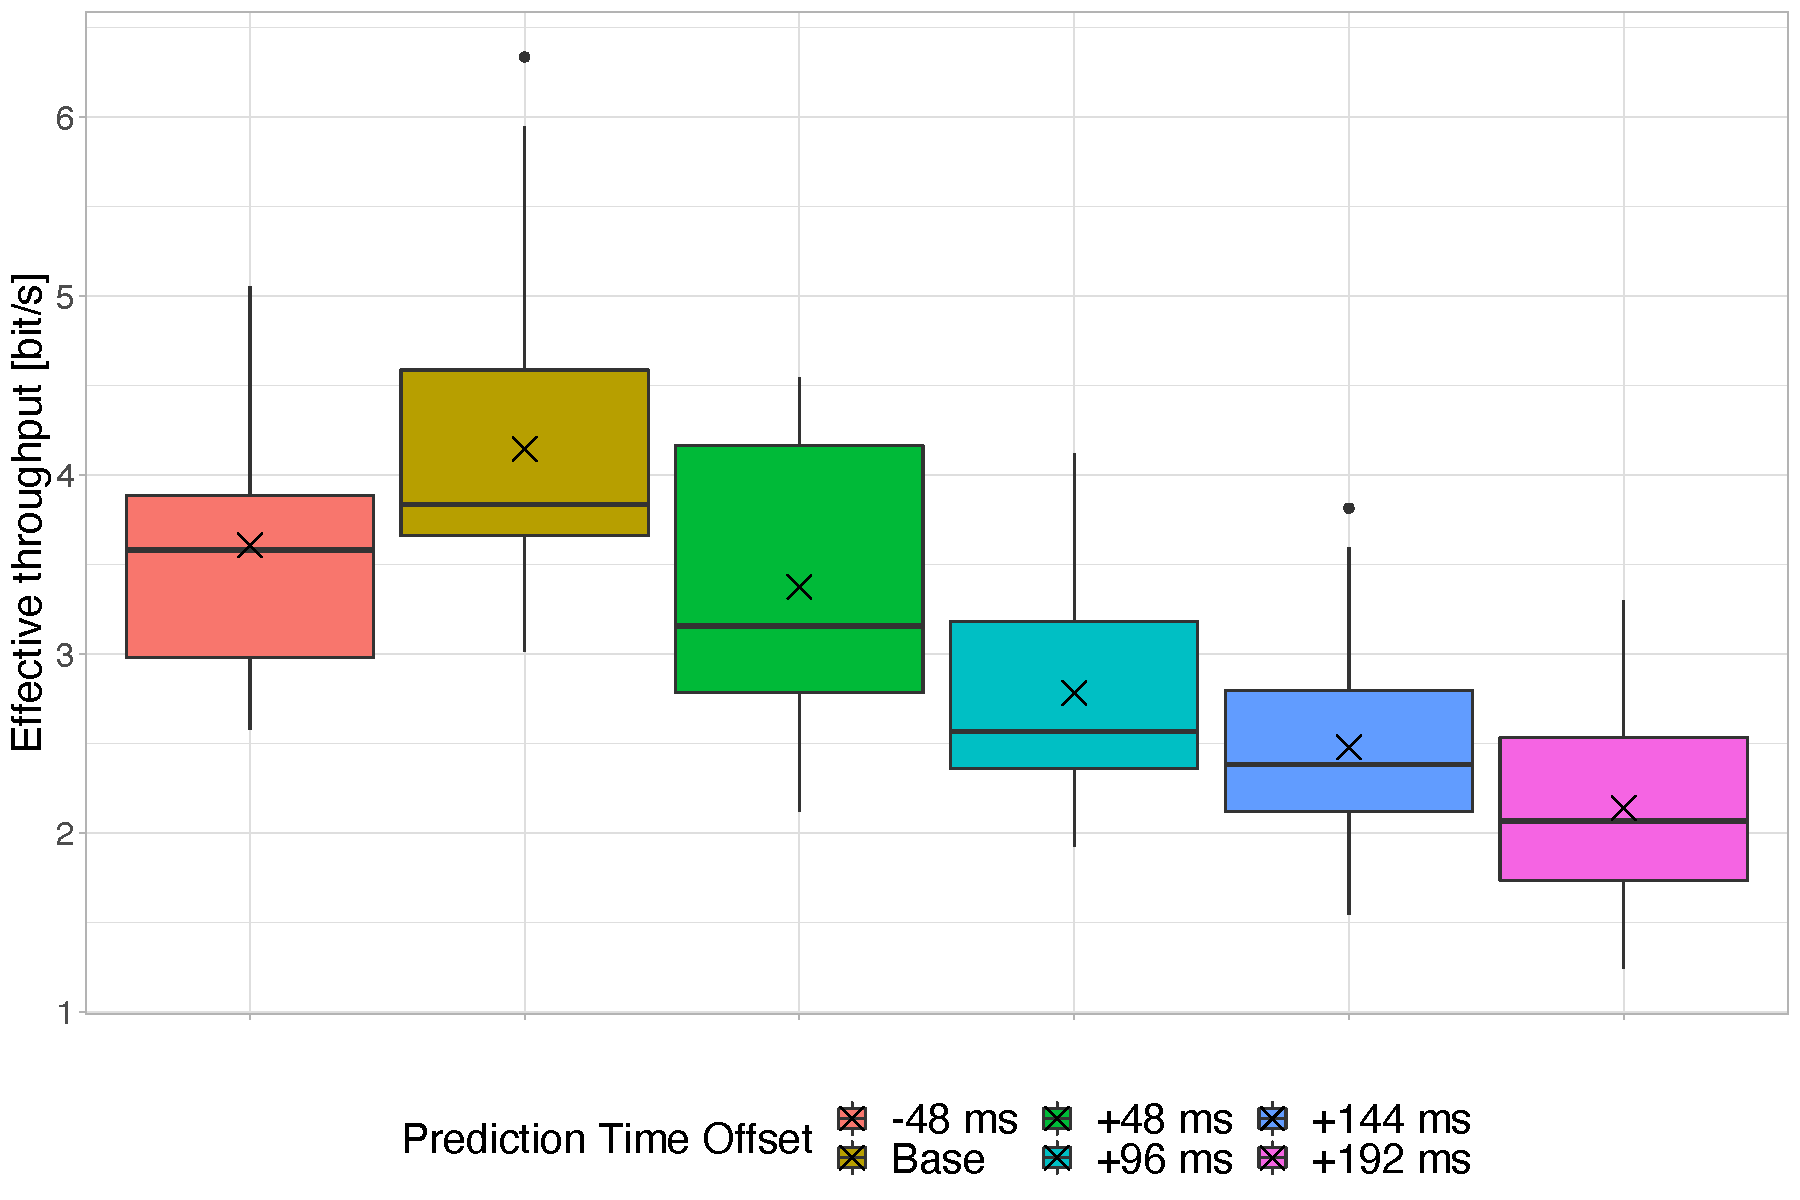
\includegraphics[width=1.0\linewidth]{boxplotchart_Throughput}
  \caption{Boxplot of the effective throughput ($TP_e$) for each  \textsc{prediction time offsets}. }
  \Description{Boxplot of the effective throughput ($TP_e$) for each  \textsc{prediction time offsets}.}
  \label{fig:bp_throughhput}
\end{figure}


Overall, harsher modifications lead to worse results. Interestingly, the pairwise Wilcoxon signed-rank test showed no significant difference between the past modification and the \textit{+48 ms model}.

It has to be noted that the throughput values observed in this study differ from other related studies, which have been conducted using a similar setup and indexes of difficulty~\cite{Schwind2019a}. Throughput values are lower here, which might indicate that participants were not successfully motivated to conduct the task as fast as possible. Another explanation might be that they were intimidated by the negative effects of the prediction models which when once observed caused them to perform slower under all conditions.\newline


\textbf{Movement Time}

The mean movement time for each participant performing a single target selection task was analyzed for the different \textsc{prediction time offsets}. Conducting Shapiro-Wilk tests on the participants mean movement times once again showed that those were not normally distributed in all of the conditions. Since prerequisites for a one way repeated-measures ANOVA were not met, the Friedmann-Test was used. Concerning movement times, there was again a significant difference between the tested groups (Friedman-Test: $\chi^2$(5) =78.41, \textit{p} < .001, n = 24).

\begin{table}
% bearbeitet
\caption{Bonferroni-adjusted \textit{p}-values of pairwise Wilcoxon signed-rank tests computed on the mean movement time.}
\Description{Bonferroni-adjusted \textit{p}-values of pairwise Wilcoxon signed-rank tests computed on the mean movement time.}
\label{table:mt_p}
\begin{tabular}{llllllll}
\toprule
         	& \multicolumn{1}{c}{Base}  & \multicolumn{1}{c}{+48 ms} 	& \multicolumn{1}{c}{+96 ms} 	& \multicolumn{1}{c}{+144 ms} 	& \multicolumn{1}{c}{+192 ms} 	\\ \midrule
-48 ms   	& \phantom{<}.08				& 1			    				& <.001****  					& <.001**** 						& <.001**** 						\\
Base     	&       						& \phantom{<}.003** 			& <.001**** 					& <.001**** 						& <.001**** 						\\
+48 ms  	&       						&        						& \phantom{<}.002** 			& \phantom{<}.001** 				& <.001***   					\\
+96 ms  	&       						&        						&            					& \phantom{<}.736				& \phantom{<}.001**     			\\
+144 ms 	&       						&        						&            					&            					& \phantom{<}.182      			\\ \bottomrule
\end{tabular}

\end{table}

Similar to the throughput, post-hot pairwise Wilcoxon signed-rank tests showed that there were significant differences for all conducted comparisons on movement time, except for the \textit{-48 ms model} compared to the \mbox{\textit{+48 ms model}} (\textit{p} = 1), the \mbox{\textit{+96 ms model}} compared to the \textit{+144 ms model}(\textit{p} = .131) and the \mbox{\textit{+144 ms model}} compared to the \mbox{\textit{+192 ms model}} (\textit{p} = .436), as can be seen in table~\ref{table:mt_p}.

\begin{figure}[H]
  \centering
  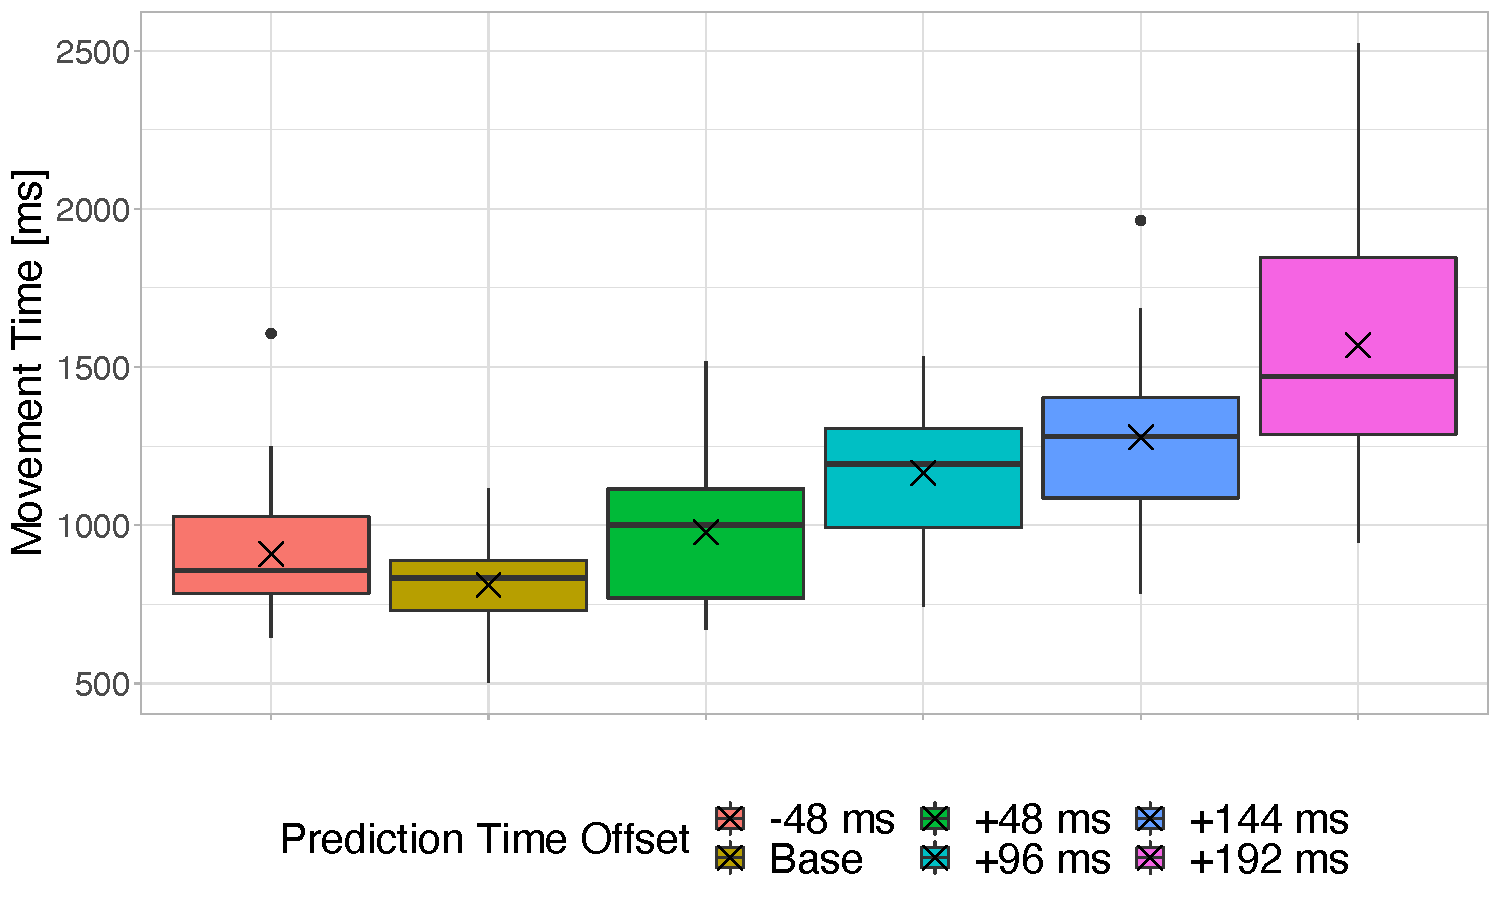
\includegraphics[width=1.0\linewidth]{boxplotchart_MovementTime}
  \caption{Boxplot of the mean movement times (\textit{MT}) for each \textsc{prediction time offsets}.}
  \Description{Boxplot of the mean movement times (\textit{MT}) for each \textsc{prediction time offsets}.}
 \label{fig:bp_movementtimes}
\end{figure}

Additionally, the comparison between the \textit{base model} and the \textit{-48 ms model} showed no significant difference this time. Using the given apparatus, the \textit{base model} had the lowest mean movement time for a single target selection task with 812 ms (\textit{SD} = 156 ms), followed by the \textit{-48 ms model} with 909 ms (\textit{SD} = 218 ms). The worst performing condition was the \mbox{\textit{+192 ms model}} with a mean movement time of 1569 ms (\textit{SD} = 444 ms). The average movement time over all conditions combined was 1119 ms (\textit{SD} = 370 ms). A visualization of the movement times for each condition can be seen in figure~\ref{fig:bp_movementtimes}.

Mean movement times were the best for the \textit{base model} and got worse for each further \textsc{prediction time offset}. As mentioned previously, the \textit{-48 ms model} produced mean movement times closest to the \textit{base model} and even outperformed the \textit{+48 ms model}.

For every \textsc{prediction time offset}, the characteristic Fitts' law linear relationship between ID and movement time can be established using linear regression models. The parameters of the linear equation indicate better performance by smaller intercepts (\textit{a} = $\beta_1$) and shallower slopes (\textit{b} = $\beta_2$)~\cite{Law2018}. Figure~\ref{fig:lin_MovementTime} shows worse performance on harsher modifications using the given apparatus. Given the stable $R^2_\text{adj}$-values and the increase in intercept as well as slope throughout the \textsc{prediction time offsets}, an overall worsening in performance can be measured.

 
\begin{figure}[H]
  \centering
  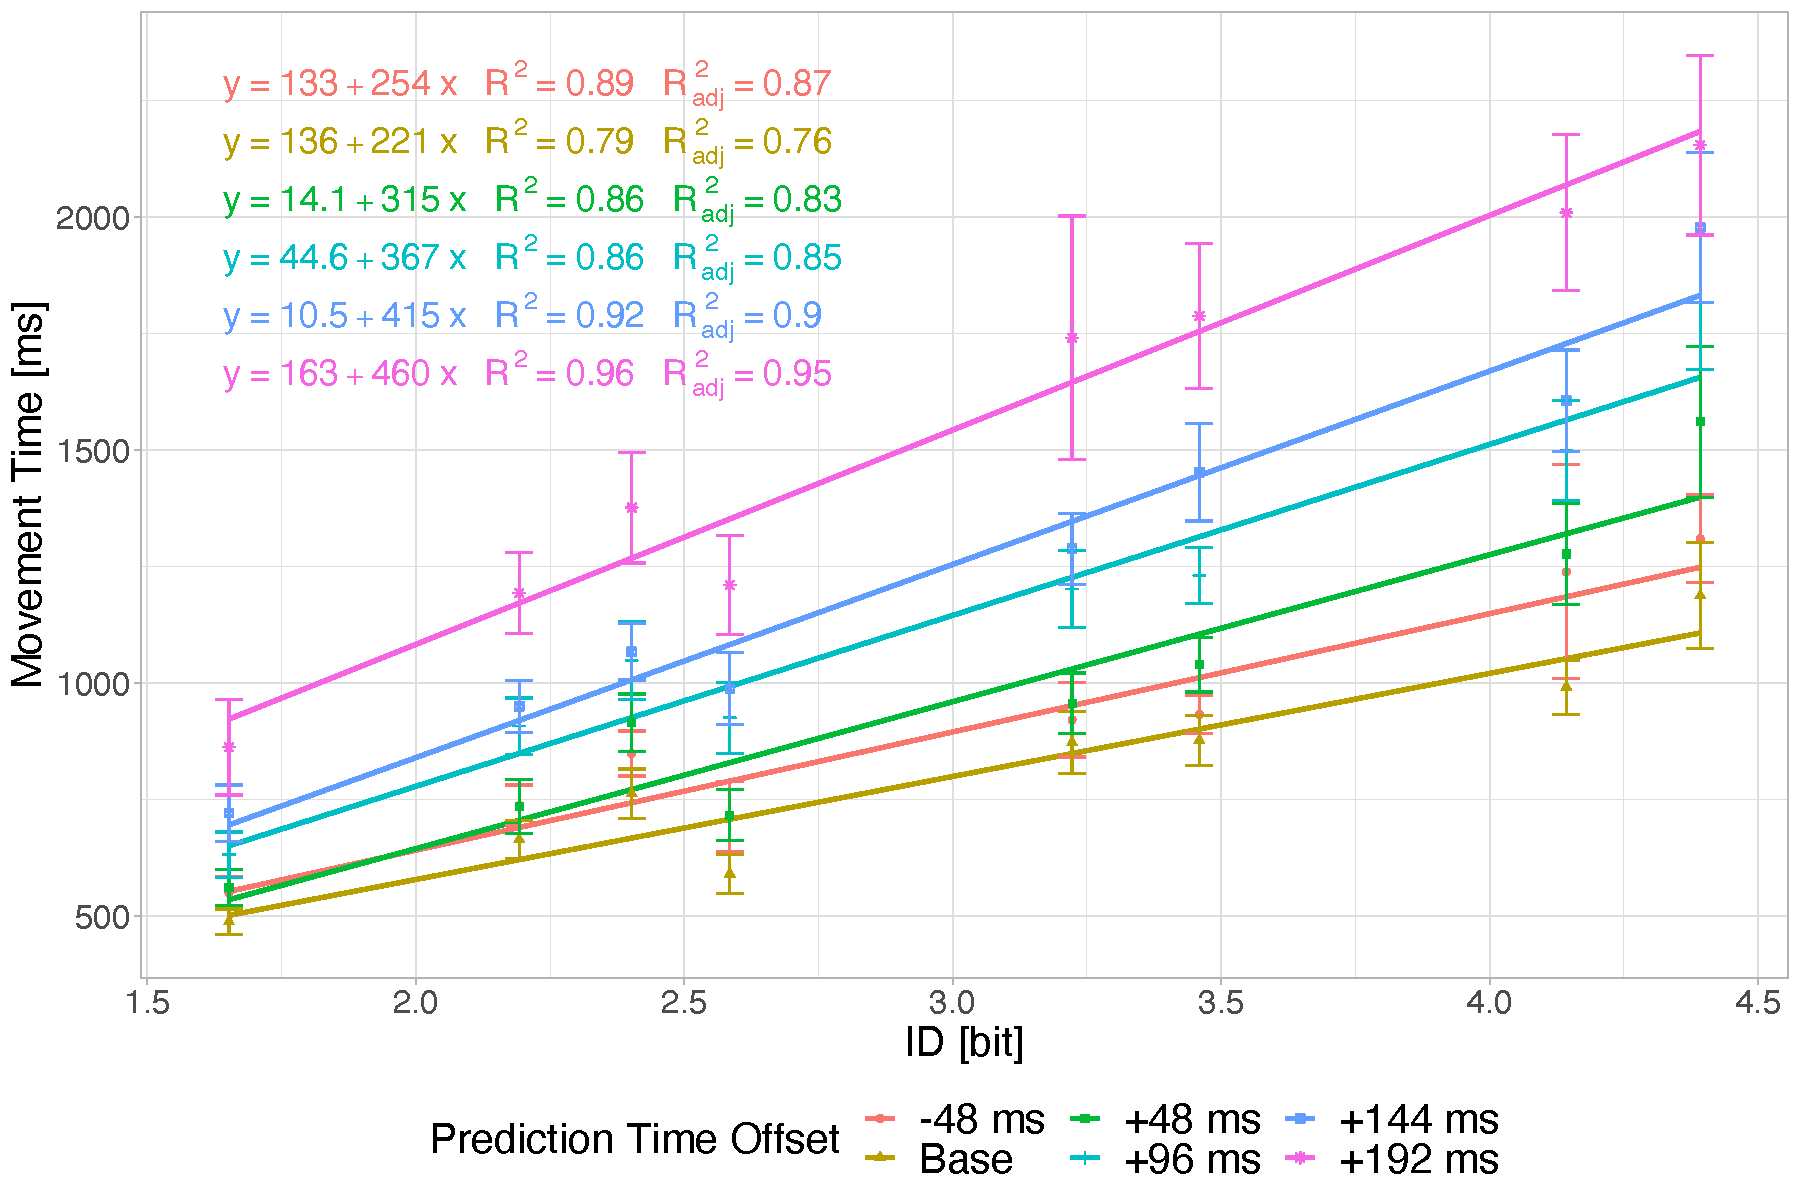
\includegraphics[width=1.0\linewidth]{lin_Movementtime_ID}
  \caption{Linear regression models for mean movement time on all \textsc{prediction time offsets} and IDs.}
  \Description{Linear regression models for mean movement time on all \textsc{prediction time offsets} and IDs.}
 \label{fig:lin_MovementTime}
\end{figure}

\textbf{Accuracy}

As a measurement of accuracy, the mean distance of the target center to the exact point where the participant hit the targets was used. 
\begin{table}[H]
\caption{Bonferroni-adjusted \textit{p}-values of pairwise Wilcoxon signed-rank tests computed on the accuracy.}
\Description{Bonferroni-adjusted \textit{p}-values of pairwise Wilcoxon signed-rank tests computed on the accuracy.}
\label{table:ac_p}
\begin{tabular}{llllllll}
\toprule
         	& \multicolumn{1}{c}{Base} 	& \multicolumn{1}{c}{+48 ms} 	& \multicolumn{1}{c}{+96 ms} 	& \multicolumn{1}{c}{+144 ms} 	& \multicolumn{1}{c}{+192 ms}    	\\ \midrule
-48 ms   	& 1							& \phantom{<}.207			 	& \phantom{<}.034*		 		& <.001**** 						& \phantom{<}.016* 					\\
Base     	&       						& \phantom{<}.291	  		 	& \phantom{<}.002** 	 		& <.001**** 						& \phantom{<}.005** 					\\
+48 ms  	&       						&        						& 1		  	 					& \phantom{<}.004**  			& \phantom{<}.144   					\\
+96 ms  	&       						&        						&            					& \phantom{<}.158     			& 1      							\\
+144 ms 	&       						&        						&            					&            					& 1      							\\ \bottomrule
\end{tabular}
\end{table}
The Shapiro-Wilk tests showed the data was not normally distributed in all of the conditions (compare table~\ref{table:ac_p}). Again, a significant difference existed between the conditions (Friedman-Test: $\chi^2$(5) =44.90, \textit{p} < .001, n = 24). Conducting the same post-hoc tests as before, significant differences were found for the \textit{-48 ms model} compared with the \mbox{\textit{+96 ms model}} (\textit{p} = .034), the \mbox{\textit{+144 ms model}} \mbox{(\textit{p} < .001)} and  the \textit{+192 ms model} (\textit{p} = .016). The \textit{Base model} also showed significant differences compared to the \mbox{\textit{+96 ms model}} (\textit{p} = .002), the \mbox{\textit{+144 ms model}} (p < .001) and  the \textit{+192 ms model} (\textit{p} = .005). The last significant difference was found between the \mbox{\textit{+48 ms model}} and the \mbox{\textit{+144 ms model}} (\textit{p} = .004). Mean distance to target center was .265 unity measures (\textit{SD} = .028).

\begin{figure}[H]
  \centering
  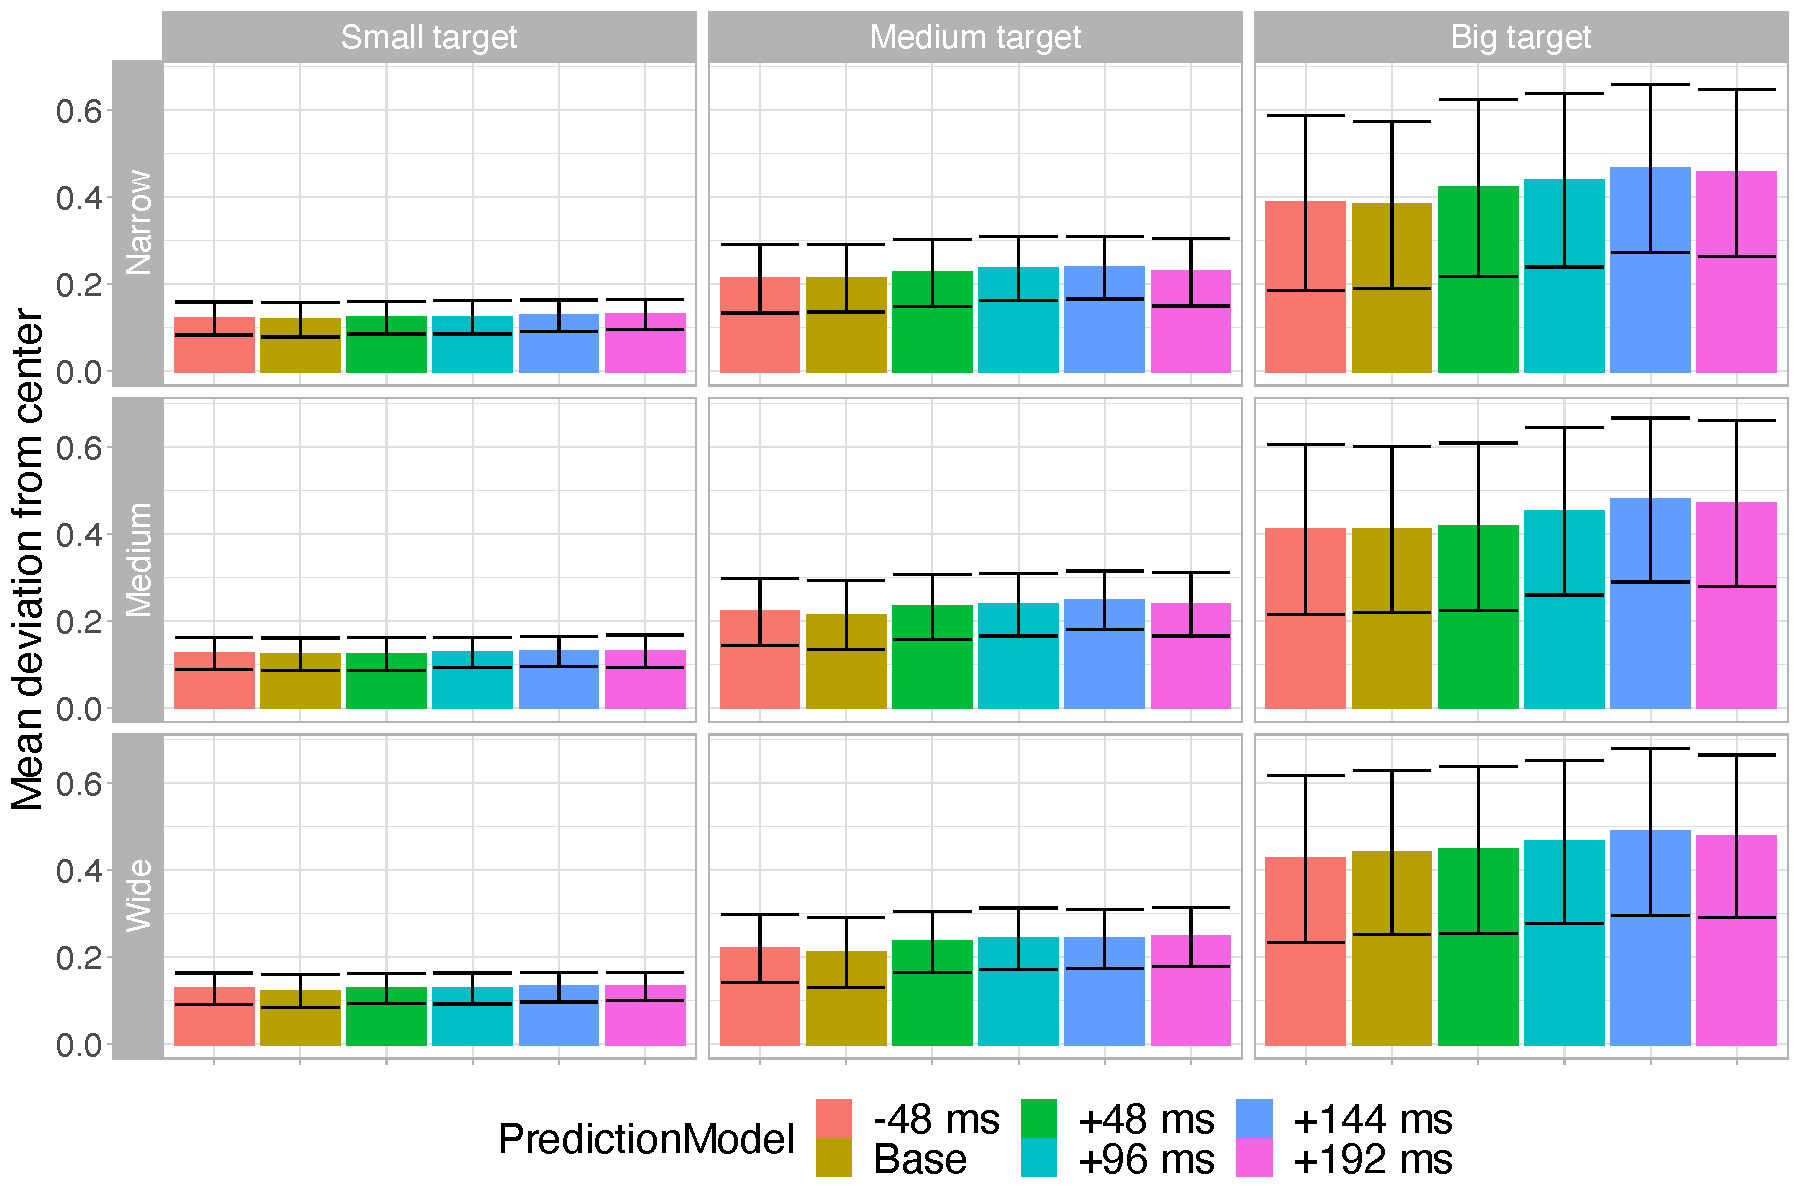
\includegraphics[width=1.0\linewidth]{Precisionplot_Barchart}
  \caption{Mean distance from selection point to target center for all featured circle configurations with their respective standard deviation.}
  \Description{Mean distance from selection point to target center for all featured circle configurations.}
  \label{fig:barchart_precision}
\end{figure}

Figure~\ref{fig:barchart_precision} displays the accuracy more precisely over all possible circle configurations. The small targets show nearly no difference in accuracy as they are as big as the avatars fingers and don't allow for much variance in selection points. The big targets as expected show the highest variance in accuracy. Although the \textsc{prediction time offsets} show similar standard deviations, different means can be observed. Accuracy seems to decline for harsher prediction modifications, suggesting similar interactions as the previous measures.
The apparatus, data and evaluation can be found on Github~\footnote{https://github.com/andreasPfaffelhuber/Faster-than-in-Real-Time}

\textbf{Questionnaires}

During the study, the participants were asked to fill out the questionnaires described in chapter~\ref{sec:Questionnaires} after each condition.
To analyze the questionnaire data, non-parametric tests were used.
This is suggested by  Gonzalez-Franco \& Peck~\cite{Gonzalez-Franco2018}, who created the avatar embodiment questionnaire used in this study, as well as common practice in other related work~\cite{Schwind2018,Lin2016}. 

%%Colors
\definecolor{C}{HTML}{0C7C59}
\definecolor{A}{HTML}{52AA5E}
\definecolor{L}{HTML}{53DD6C}
\definecolor{O}{HTML}{BEEF9F}
\definecolor{I}{HTML}{89AAE6}
\definecolor{M}{HTML}{F6AE2D}

\newcommand{\colWidth}{1.1cm}

\newcolumntype{P}[1]{>{\centering\arraybackslash}p{#1}}
\newcolumntype{P}[1]{>{\centering\arraybackslash}p{#1}}


\begin{table*}
\caption{Bonferroni-adjusted \textit{p}-values of pairwise Wilcoxon signed-rank tests for all questionnaires.\\ (\colorbox{I}{presence},\colorbox{M}{motion sickness}, \colorbox{C}{avatar embodiment},\colorbox{A}{"agency and motor control"},\colorbox{L}{"location of the body"},\colorbox{O}{"body ownership"})}

\sisetup{table-format = -1.3, table-number-alignment = center, table-space-text-pre = (, table-align-text-pre = false, table-space-text-post = {***}}
\setlength{\tabcolsep}{5pt}

\label{tab:commands}
\begin{tabularx}{16cm}{XXXXXXXXXXXXX}
\hline
                        & \multicolumn{2}{c}{-48 ms} 				& \multicolumn{2}{c}{Base} 					& \multicolumn{2}{c}{+48 ms} 								& \multicolumn{2}{c}{+96 ms} 				& \multicolumn{2}{c}{+144 ms} 					& \multicolumn{2}{c}{+ 192 ms}  				\\ \hline
\multirow{2}{*}{-48 ms}  &				&  				 			&\cellcolor{C}1& \cellcolor{A}1				&\cellcolor{C}1& \cellcolor{A}1 								&\cellcolor{C}\phantom{<}.021* & \cellcolor{A}\phantom{<}.024*   &\cellcolor{C}<.001***& \cellcolor{A}\phantom{<}.066\phantom{<} 		&\cellcolor{C}<.001*** & \cellcolor{A}\phantom{<}.003**	\\
                         &				& 							&\cellcolor{L}1& \cellcolor{O}1 				&\cellcolor{L}1 & \cellcolor{O}1    							&\cellcolor{L}1 & \cellcolor{O}\phantom{<}.046      	&\cellcolor{L}\phantom{<}.005**& \cellcolor{O}\phantom{<}.022*		&\cellcolor{L}\phantom{<}.003** & \cellcolor{O}<.001***	\\
\multirow{2}{*}{Base}    &\multicolumn{2}{c}{\cellcolor{I}1\phantom{<<<<<}}			&			   & 							&\cellcolor{C}\phantom{<}.153 & \cellcolor{A}\phantom{<}.117	&\cellcolor{C}\phantom{<}.009** & \cellcolor{A}\phantom{<}.016*	&\cellcolor{C}<.002** & \cellcolor{A}\phantom{<}.011*	&\cellcolor{C}<.001***& \cellcolor{A}<.001***  	\\
                       	 &\multicolumn{2}{c}{\cellcolor{M}1\phantom{<<<<<}}			&			   & 			 				&\cellcolor{L}1 & \cellcolor{O}\phantom{<}.464								&\cellcolor{L}1 & \cellcolor{O}\phantom{<}.06 		&\cellcolor{L}\phantom{<}.018*& \cellcolor{O}\phantom{<}.018*			&\cellcolor{L}\phantom{<}.005** & \cellcolor{O}<.001***  	\\
\multirow{2}{*}{+48 ms}  &\multicolumn{2}{c}{\cellcolor{I}1\phantom{<<<<<}}			&\multicolumn{2}{c}{\cellcolor{I}1\phantom{<<<<<}}			&			   	& 			 								&\cellcolor{C}\phantom{<}.465 & \cellcolor{A}\phantom{<}.255	&\cellcolor{C}\phantom{<}.102* & \cellcolor{A}\phantom{<}.926			&\cellcolor{C}\phantom{<}.07** & \cellcolor{A}\phantom{<}.001*  	\\
                         &\multicolumn{2}{c}{\cellcolor{M}1\phantom{<<<<<}}			&\multicolumn{2}{c}{\cellcolor{M}1\phantom{<<<<<}}	 		&				& 			     							&\cellcolor{L}1 & \cellcolor{O}.87    		&\cellcolor{L}\phantom{<}.005** & \cellcolor{O}1		&\cellcolor{L}\phantom{<}.005** & \cellcolor{O}\phantom{<}.026*  	\\
\multirow{2}{*}{+96 ms}  &\multicolumn{2}{c}{\cellcolor{I}1\phantom{<<<<<}}		&\multicolumn{2}{c}{\cellcolor{I}1\phantom{<<<<<}}			&\multicolumn{2}{c}{\cellcolor{I}1\phantom{<<<<<}}							&				& 				    		&\cellcolor{C}\phantom{<}.92 & \cellcolor{A}1  			&\cellcolor{C}\phantom{<}.002** & \cellcolor{A}\phantom{<}.113  		\\
                       	 &\multicolumn{2}{c}{\cellcolor{M}1\phantom{<<<<<}}		&\multicolumn{2}{c}{\cellcolor{M}1\phantom{<<<<<}}		&\multicolumn{2}{c}{\cellcolor{M}\phantom{<}.128\phantom{<}}			&				& 				    		&\cellcolor{L}\phantom{<}.003** & \cellcolor{O}1  			&\cellcolor{L}\phantom{<}.006** & \cellcolor{O}<.001***  	\\
\multirow{2}{*}{+144 ms} &\multicolumn{2}{c}{\cellcolor{I}\phantom{<}.859\phantom{<}}		&\multicolumn{2}{c}{\cellcolor{I}\phantom{<}.321\phantom{<}}		&\multicolumn{2}{c}{\cellcolor{I}1\phantom{<<<<<}}							&\multicolumn{2}{c}{\cellcolor{I}1\phantom{<<<<<}}			&				& 								&\cellcolor{C}\phantom{<}.032* & \cellcolor{A}\phantom{<}.348  		\\
                         &\multicolumn{2}{c}{\cellcolor{M}\phantom{<}.784\phantom{<}}		&\multicolumn{2}{c}{\cellcolor{M}\phantom{<}.274\phantom{<}}		&\multicolumn{2}{c}{\cellcolor{M}\phantom{<}.109\phantom{<}}   			&\multicolumn{2}{c}{\cellcolor{M}1\phantom{<<<<<} }      	&				&								&\cellcolor{L}1 & \cellcolor{O}\phantom{<}.008**  			\\ 
\multirow{2}{*}{+192 ms} &\multicolumn{2}{c}{\cellcolor{I}\phantom{<}.071\phantom{<}}		&\multicolumn{2}{c}{\cellcolor{I}\phantom{<}.03*\phantom{<}}		&\multicolumn{2}{c}{\cellcolor{I}\phantom{<<}.146\phantom{<}}			&\multicolumn{2}{c}{\cellcolor{I}\phantom{<}.095\phantom{<}}		&\multicolumn{2}{c}{\cellcolor{I}\phantom{<}.61}				&				&	  							\\
                         &\multicolumn{2}{c}{\cellcolor{M}\phantom{<}.149\phantom{<}}		&\multicolumn{2}{c}{\cellcolor{M}\phantom{<}.081\phantom{<}}		&\multicolumn{2}{c}{\cellcolor{M}\phantom{<}.022*}   			&\multicolumn{2}{c}{\cellcolor{M}\phantom{<}.594\phantom{<}}   	&\multicolumn{2}{c}{\cellcolor{M}1}  			&				&  								\\\hline
\end{tabularx}	
\label{table:q_p}	
\end{table*}

Values of the iPQ are computed by using the mean of all involved items. Results for the avatar embodiment and the used sub-scales in "body ownership", "agency and motor control" as well as "location of the body" are calculated using the equations presented by its authors~\cite{Gonzalez-Franco2018}.The motion sickness is computed using the mean of all involved items.
%% \textit{p}-values for the post-hoc tests on all questionnaires can be seen in table~\ref{table:q_p}.

%% IPQ
When evaluating the iPQ on presence a significant difference existed between the conditions (Friedman-Test: $\chi^2$(5) = 20.1, \mbox{\textit{p} < .05}, n = 24).
The post-hoc tests resulted in no significant differences between the conditions except for the \textit{base model} and the \mbox{\textit{+192 ms model}} (\mbox{\textit{p} = .03})

%% but on \textit{-48 ms model} and \mbox{\textit{+192 ms model}} (\mbox{\textit{p} = .042}) as well as \textit{base model} and \mbox{\textit{+192 ms model}} (\textit{p} = .027). This does not support the expectation of changing perception of presence along the different \textsc{prediction time offsets}.
	
%% EQ	
Evaluating the avatar embodiment resulted in significant differences between multiple conditions (Friedman-Test: $\chi^2$(5) = 51.3, \mbox{\textit{p} < .05}, n = 24). 

%% EQ A
When evaluating the Avatar Embodiment sub-scales significant differences could be found for
"agency and motor control" (Friedman-Test: $\chi^2$(5) = 47.8, \textit{p} < .05, n = 24),
"body ownership" (Friedman-Test: $\chi^2$(5) = 49.7, \textit{p} < .05, n = 24). as well as 
"location of the body" (Friedman-Test: $\chi^2$(5) = 41.4, \textit{p} < .05, n = 24). Overall the sub-scales resemble the avatar embodiment scale. More drastic changes report worse avatar embodiment scores.  
	
%% MS
The motion sickness questions found significant differences between some groups (Friedman-Test: $\chi^2$(5) = 25.7, \textit{p} < .005, n = 24), though only between the \textit{+48 ms model} and \textit{+192 ms model} (\textit{p} = .022) was reported by the Wilcoxon signed-rank test. Overall participants didn't report effects of motion sickness regardless of the \textsc{prediction time offset}, though a slight increase of the means towards the harsher \textsc{prediction time offsets} indicates that those overstepped the boundary of subjectively pleasant motion alteration.

\begin{figure}
  \centering
  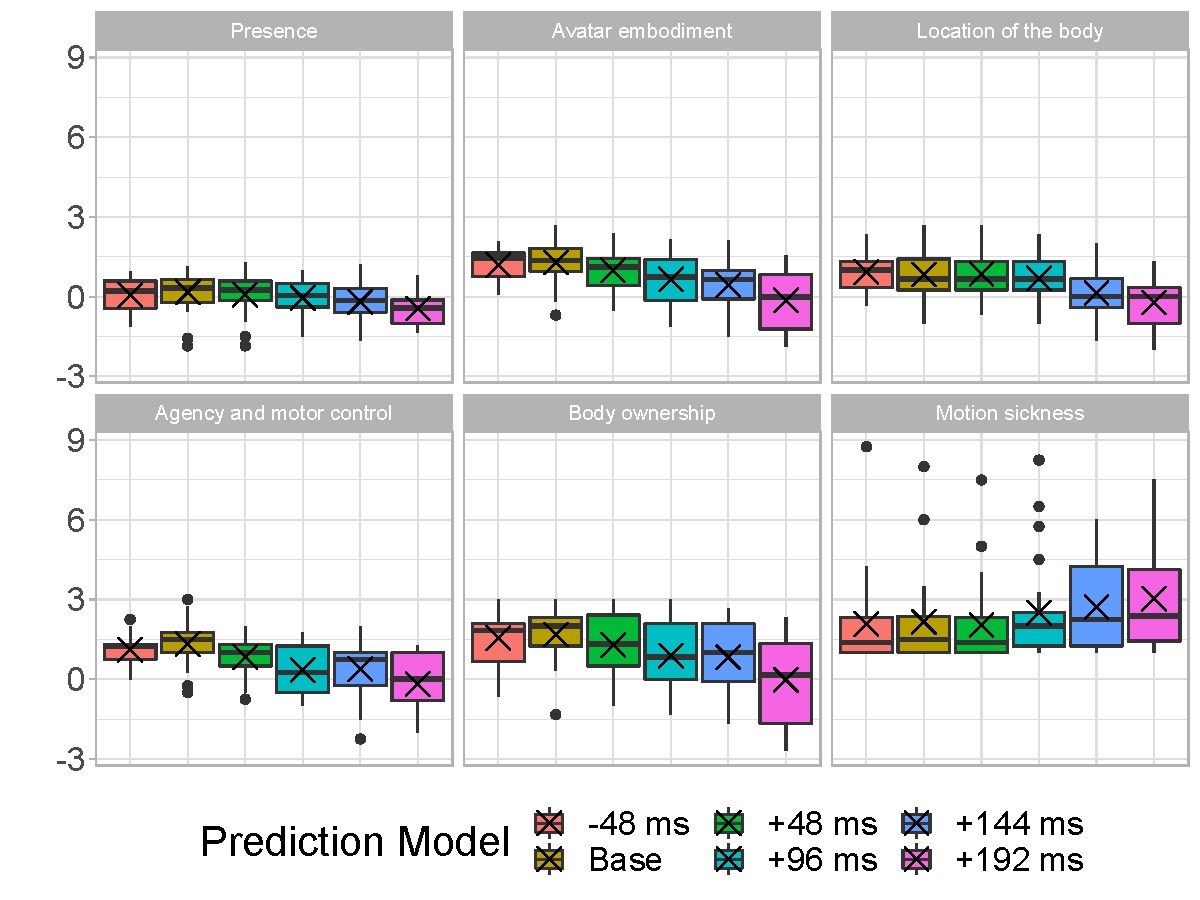
\includegraphics[width=1.0\linewidth]{boxplotchart_allQuestionnaires}
  \caption{Function fit and mean movement time for all \textsc{prediction time offsets} and IDs.}
  \Description{Function fit and mean movement time for all \textsc{prediction time offsets} and IDs.}
\end{figure}


\textbf{Qualitative Feedback}

The qualitative feedback given after each condition was analyzed in order to gain further insight on how participants perceived the different \textsc{prediction time offsets}. Participants had only been told they were testing different tracking configurations during the study, and had answered the questions described in chapter~\ref{sec:Questionnaires} in a thinking aloud manner. Considering the \mbox{\textit{+96 ms model}} and the even more intense prediction models, nearly all participants reported that they did not find those to function particularly well. They reported that the hand of the digital avatar was shaking as well as jumping around most of the time, that moving the avatar felt a bit uncontrollable, and that precise selections were nearly impossible to do. Those factors seemed to generally get worse using stronger \textsc{prediction time offsets}. As a result, most participants reported to feel that the currently tested condition was working pretty bad, and that they did not feel as if the avatar resembled their real body and its motions. 
The \mbox{\textit{+48 ms model}}, the \textit{base model} and the \mbox{\textit{-48 ms model}} were rated much better compared to the previously described ones. Participants did usually not perceive the negative effects listed for the other models, but reported much more smooth and congruent motions. Interestingly, participants rated the \mbox{\textit{+48 ms model}}, \mbox{\textit{base model}} and the \mbox{\textit{-48 ms model}} very similar. Many participants noted that their motions felt either somewhat slow or a little bit sped up when compared to their experience with the baseline system or the other mentioned model, but didn't agree on which model caused which effect. While some participants reported the \mbox{\textit{+48 ms model}} was speeding up their motions and the past model was slowing them down, others had the exact opposite impressions. We suspect that a possible explanation for this might be that reverting the motion's direction could take longer using future prediction, since the movement would continue in the original direction for a bit even if the participants hand never did, maybe even longer than when buffering the past frames. 

The base system without any prediction was the one most participants rated as their favorite condition, often stating that it offered the best direct translation of their real motions to the avatar's motions and lacked the negative effects of the future prediction.

\section{Discussion}\label{tit:Discussion}

In this study, employing neural networks to predict user motions using different \textsc{prediction time offsets} has been investigated. Additionally, the baseline model as well as a past time model using buffered frames were used to further validate the findings and to quantitatively model the occurred prediction effect. A standardized two-dimensional Fitts' law task was conducted to compare user performance in the virtual environment.
The initial expectations were that the smaller future prediction models would result in a better user performance and presence than the past and the baseline model, before those would drop off again due to the stronger prediction models over-predicting the participants motions. 
Statistical evaluations concerning the performance measures show the overall existence of significant differences between the different \textsc{prediction time offsets}. Throughput, movement time and accuracy all confirm that the used model makes a difference, yet the observed differences are not at all like initially expected.
The expected improvement using future and therefore faster versions of the motions could not be observed. Instead we found a negative influence using stronger changes, with even the smallest model already negatively impacting all of the performance measures compared to the \textit{base system}. 
Questionnaire data collected during the study confirms that the avatar embodiment as well as as the connected sub-scales show similar trends as the performance measures. 
Presence as computed by the iPQ on the other hand was not affected by the described setup and conditions. No significant difference was observed except once for the harshest motion alteration. 

One possible explanation for the observed results might be that future motions generally make participants perform worse since they notice that their real-world motions are not congruent with the avatars motions observed in the virtual environment. Participants could thus intuitively slow down their motions simply because of the decrease in avatar embodiment and limb-ownership, due to the translation not being entirely correct and resulting in a difference between their expected virtual limb position and the out-coming one. Therefore, even a theoretically perfect prediction of a user's movement might not increase performance as users could be too cautious or possibly overshoot due to the prediction continuing in movement direction for a little while longer.

Another possible explanation could be that the trained prediction models did not reach the necessary amount of accuracy to really speed up user motions correctly. Shaking limbs or too inaccurate predictions of their motions also would require the participants to spend time correcting their avatar positions and could result in lower performance in the given Fitts' law task. Qualitative data captured during the experiment would at least confirm this suspicion for the worst prediction models, where participants often complained about these negative effects. 

\textbf{Limitations and Future Work}

Given the hardware setup and the high frame-rate of the motion tracking system, the used neural network architecture was limited by computation time. This resulted in the use of a shallow architecture, which does not work on time sequences. Using more capable hardware, network architectures like recurrent neural networks (RNN) which allow for time sequences~\cite{Martinez2017} might lead to a more stable motion prediction and thus better results.

Additionally, in the current setup only general prediction models were used. Training data was not specifically captured for the sitting Fitts' law task and thus the models are not optimized for the given task.

Future work might want to explore whether specifically captured data and better hardware allow more accurate models resulting in better user performance and better embodiment. Additionally, the study only tested one experimental setup where all participants conducted the task on an horizontal axis sitting at a table. Since virtual reality environments and the used motion capture system would theoretically allow for motions along other directions as well, different free standing or moving configurations not only focusing on a table setup could be evaluated as well. This might provide a better well-rounded insight instead of limiting the findings to a rather specific set of tasks.

%%
%% The next two lines define the bibliography style to be used, and
%% the bibliography file.
\bibliographystyle{ACM-Reference-Format}
\bibliography{PS_1}

\end{document}
\endinput
%%
%% End of file `sample-authordraft.tex'.
\bibliography{sample-base}